%% ==============
\chapter{Leichtgewichtige Generierung mit InstaGuide}
\label{ch:Instaguide}
%% ==============

Mit Hilfe von  Modell-zu-Modell-Transformationen kann der Zustand
eines Systems in einer anderen Form dargestellt werden.

Textuelle Handb�cher automatisch generieren
Modell der Systembeschreibung als Ausgangspunkt

Meta-Informationen aus einem separaten Model entnehmen

Automatisierungsgrad hoch halten


Der Transformationsmechanismus ist automatisiert 

Herausforderungen sind es eine Transformation zu erstellen die ein f�r
den Menschen nutzbares Resultat liefert und auch schnell genug
l�uft um sie mit jeder �nderung neu generieren zu k�nnen.

Die Erkundungsphase, in der ein �berblick �ber das System und dessen
Komponenten gegeben wird, kann mit Hilfe eine Online-Konfigurators
ersetzt werden. Dem Benutzer wird das System im ganzen Pr�sentiert und
er hat die M�glichkeit die Komponenten auszuw�hlen die ihn
interessieren. Wird der Konfigurator benutzt kann automatisch f�r
jeden Kunden eine Feature-Liste erstellt werden. Aus dieser
Feature-Liste entsteht eine Variante des Produktes aus der das
Handbuch generiert werden soll.

Relations between components on a meta level have do be defined, or do
they?
Consider having dependencies, they must be known within the system
model (Uses relations)


\begin{figure}[htb]
  \centering
  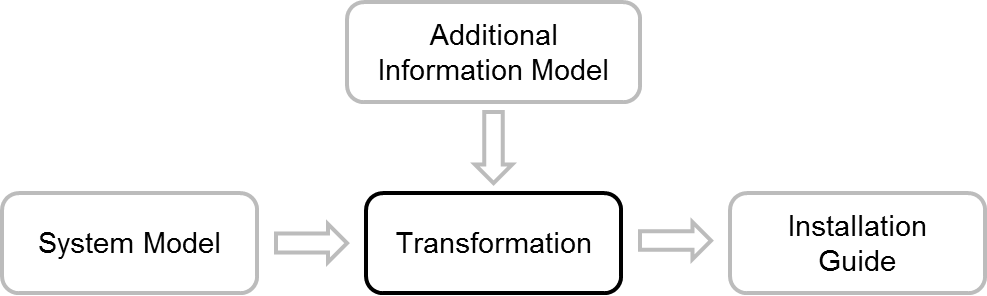
\includegraphics[width=0.8\textwidth]{img/instaguide-basic_overview.png}
  \caption{Instaguide-Ansatz �berblick}
  \label{fig:instaguide-ueberblick}
\end{figure}

In dem Beispielszenario


\begin{table}
  %\rowcolors{3}{green!25}{yellow!50}
  \caption{Vergleich der Ans�tze(unter dem Aspekt der Benutzbarkeit)}
  \centering
  \begin{tabular}{l c c c c c}
    %heading
    \hline\hline
    
    & Licht & \\ [1ex]

    \hline
    %heading end
	
	Heizk�rper & $\times$ & \checkmark \\ [1ex]
	LED Strang \\ [1ex]
	Steckdosen \\ [1ex]
	Server \\ [1ex]
    \hline
  \end{tabular}
  \label{table:tab1}
\end{table}


User stories:
User buys some of the gizmos we offer
In the background the configuration has to check the constraints
User gets the package and a QR code to read in with the app(offline for mounting when data connection available)


Nat�rliche Sprache 
